%**************************************************************************************
% License:
% CC BY-NC-SA 4.0 (http://creativecommons.org/licenses/by-nc-sa/4.0/)
%**************************************************************************************

\documentclass[beamer]{beamer}

\mode<presentation> {

\usetheme{Madrid}

% Burnt orange
\definecolor{burntorange}{rgb}{0.8, 0.33, 0.0}
\colorlet{beamer@blendedblue}{burntorange}
% Pale yellow
\definecolor{paleyellow}{rgb}{1.0, 1.0, 0.953}
\setbeamercolor{background canvas}{bg=paleyellow}
% Secondary and tertiary palett
\setbeamercolor*{palette secondary}{use=structure,fg=white,bg=burntorange!80!black}
\setbeamercolor*{palette tertiary}{use=structure,fg=white,bg=burntorange!60!black}

% To remove the footer line in all slides uncomment this line
%\setbeamertemplate{footline}
% To replace the footer line in all slides with a simple slide count uncomment this line
%\setbeamertemplate{footline}[page number]

% To remove the navigation symbols from the bottom of all slides uncomment this line
%\setbeamertemplate{navigation symbols}{}
}

\usepackage{amsmath}
\usepackage{graphicx} % for figures
\usepackage{subcaption} % for subplots 
\usepackage[labelsep=space,tableposition=top]{caption}
\renewcommand{\figurename}{Fig.} 
\usepackage{cleveref}
\usepackage{booktabs} % Allows the use of \toprule, \midrule and \bottomrule in tables

%----------------------------------------------------------------------------------------
%	TITLE PAGE
%----------------------------------------------------------------------------------------
% The short title appears at the bottom of every slide, the full title is only on the title page
\title[CE394M: Geotechnical modeling]{CE394M: Advanced Analysis in Geotechnical Engineering} 

\author{Krishna Kumar} % name
\institute[UT Austin] % institution 
{
University of Texas at Austin \\
\medskip
\textit{
  \url{krishnak@utexas.edu}} % Your email address
}
\date{\today} % Date, can be changed to a custom date

\begin{document}

\begin{frame}
\titlepage % title page as the first slide
\end{frame}

\begin{frame}
 % Table of contents slide, comment this block out to remove it
 \frametitle{Overview}
 % Throughout your presentation, if you choose to use \section{} and \subsection{} 
 % commands, these %will automatically be printed on this slide as an overview 
 \tableofcontents
\end{frame}

%----------------------------------------------------------------------------------------
% slides
%----------------------------------------------------------------------------------------

%------------------------------------------------
\section{Geotechnical modeling}
%------------------------------------------------

\subsection{Complexity in Geotechnical modeling}
%------------------------------------------------
\begin{frame}
\frametitle{Geotechnical modeling of the complex world}
\begin{figure}
	\mode<beamer>{
		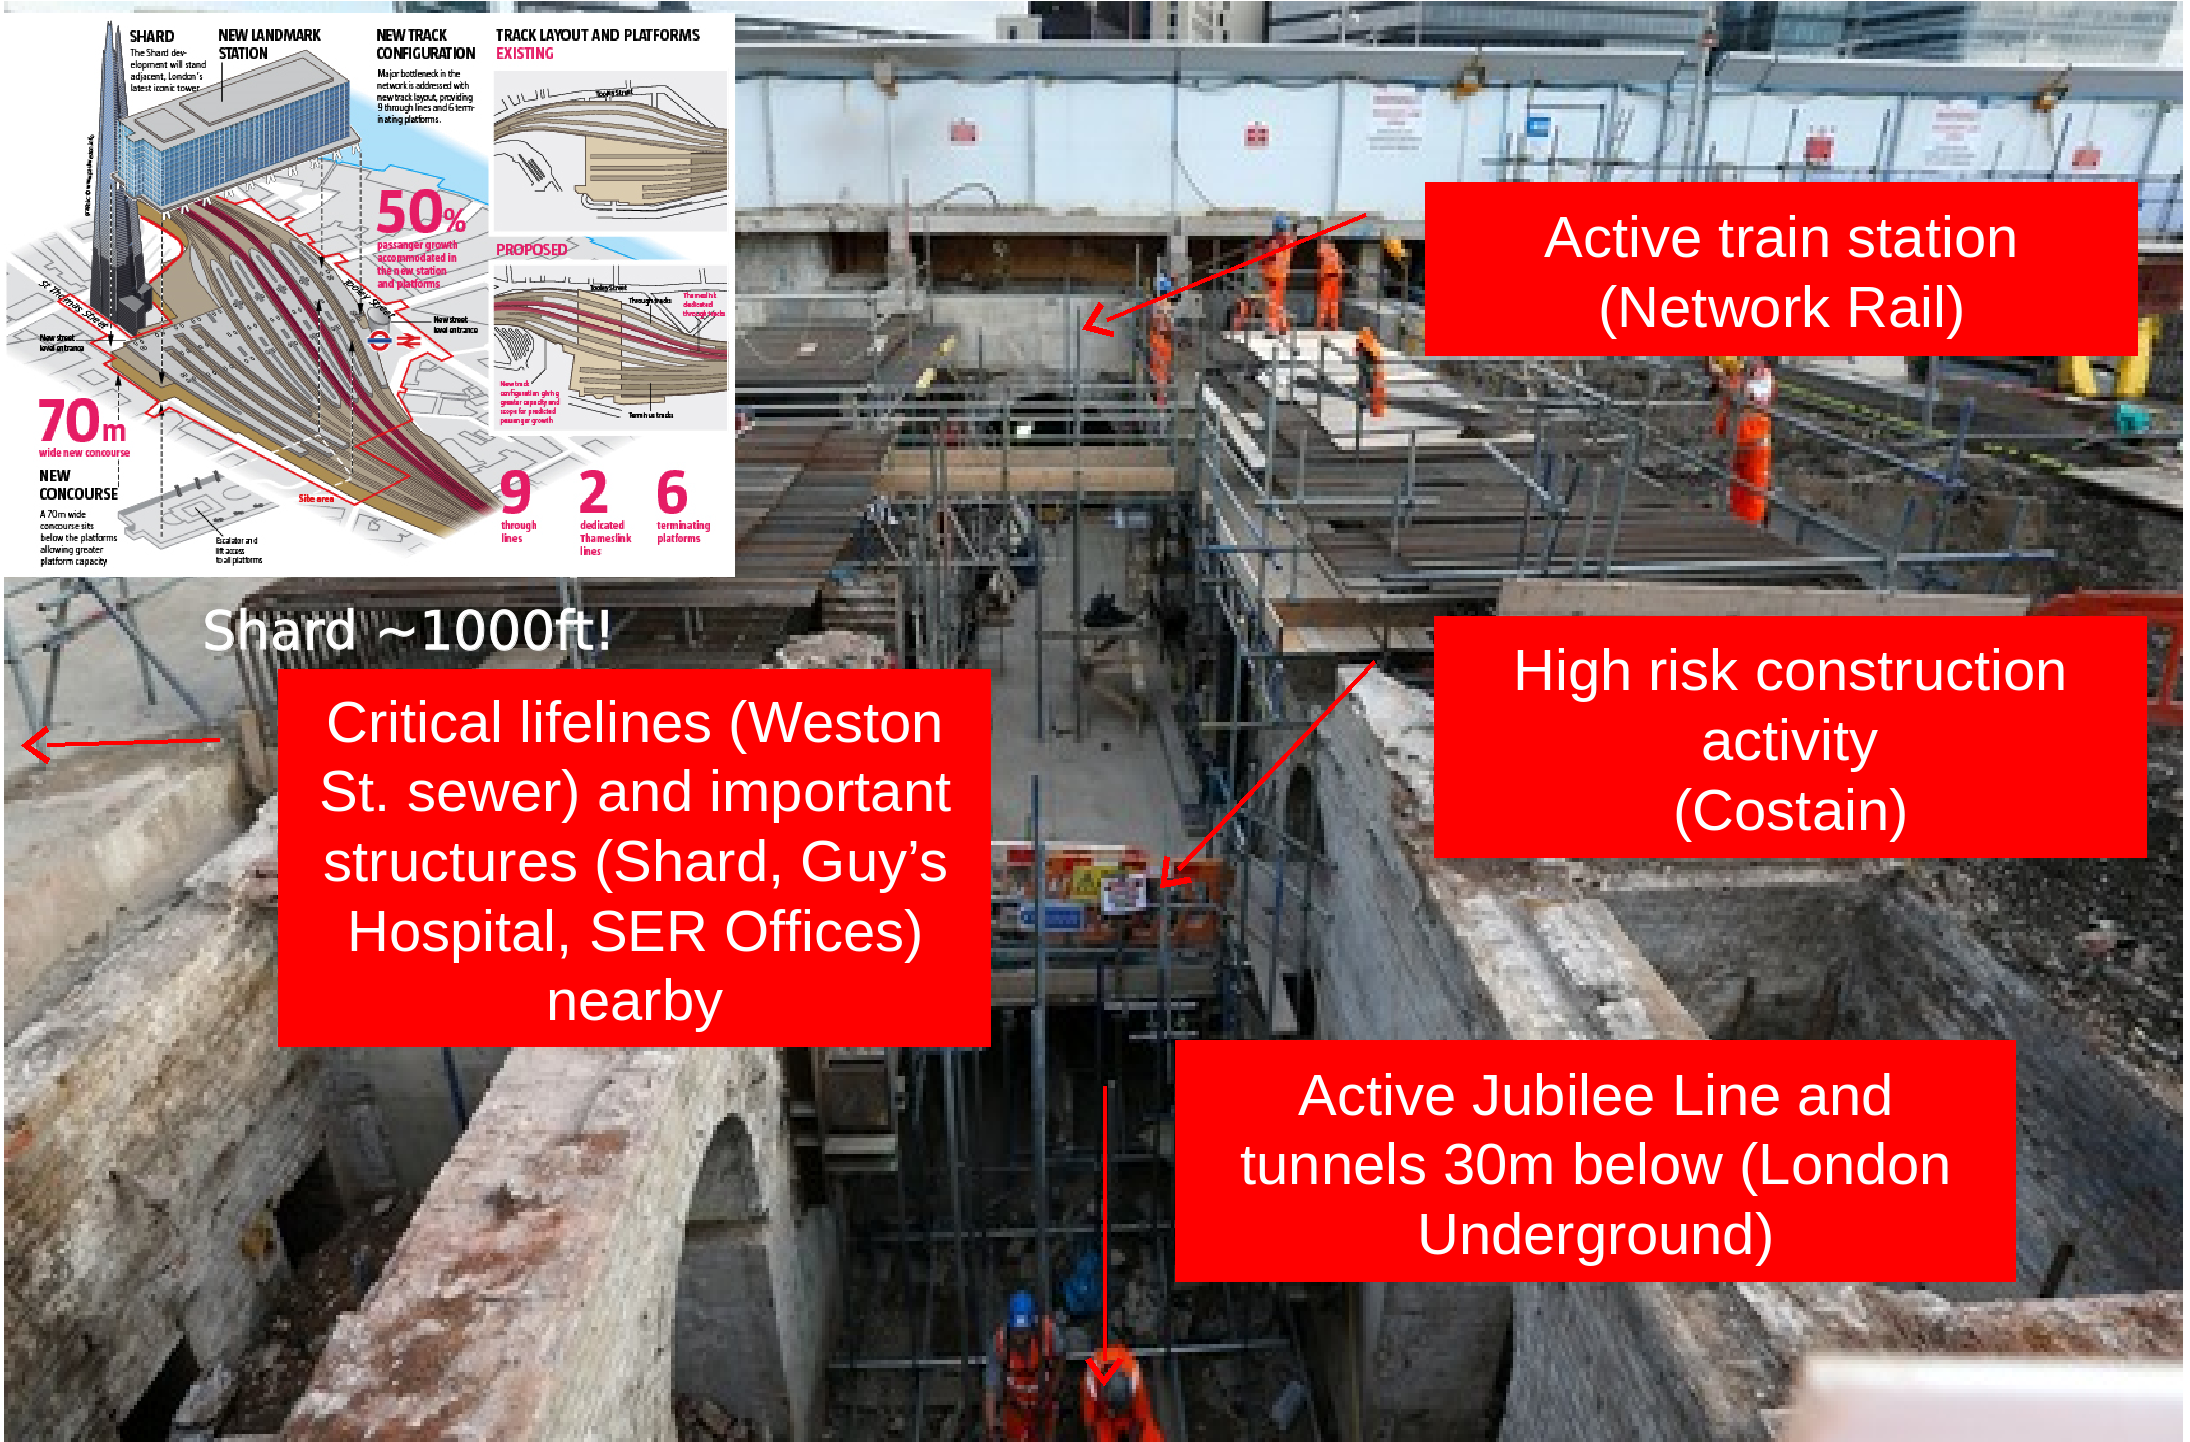
\includegraphics[width=0.85\textwidth]{figs/lbs.png}
	}
	\mode<handout>{
		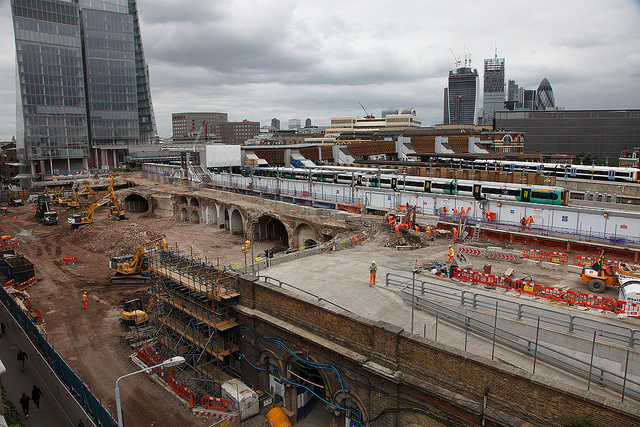
\includegraphics[width=0.85\textwidth]{figs/lbs-overview.jpg}
	}
	\caption{London Bridge Station, London, UK}
\end{figure}
\end{frame}

%------------------------------------------------
\begin{frame}
\frametitle{Geotechnical modeling of the complex world}
\begin{figure}
	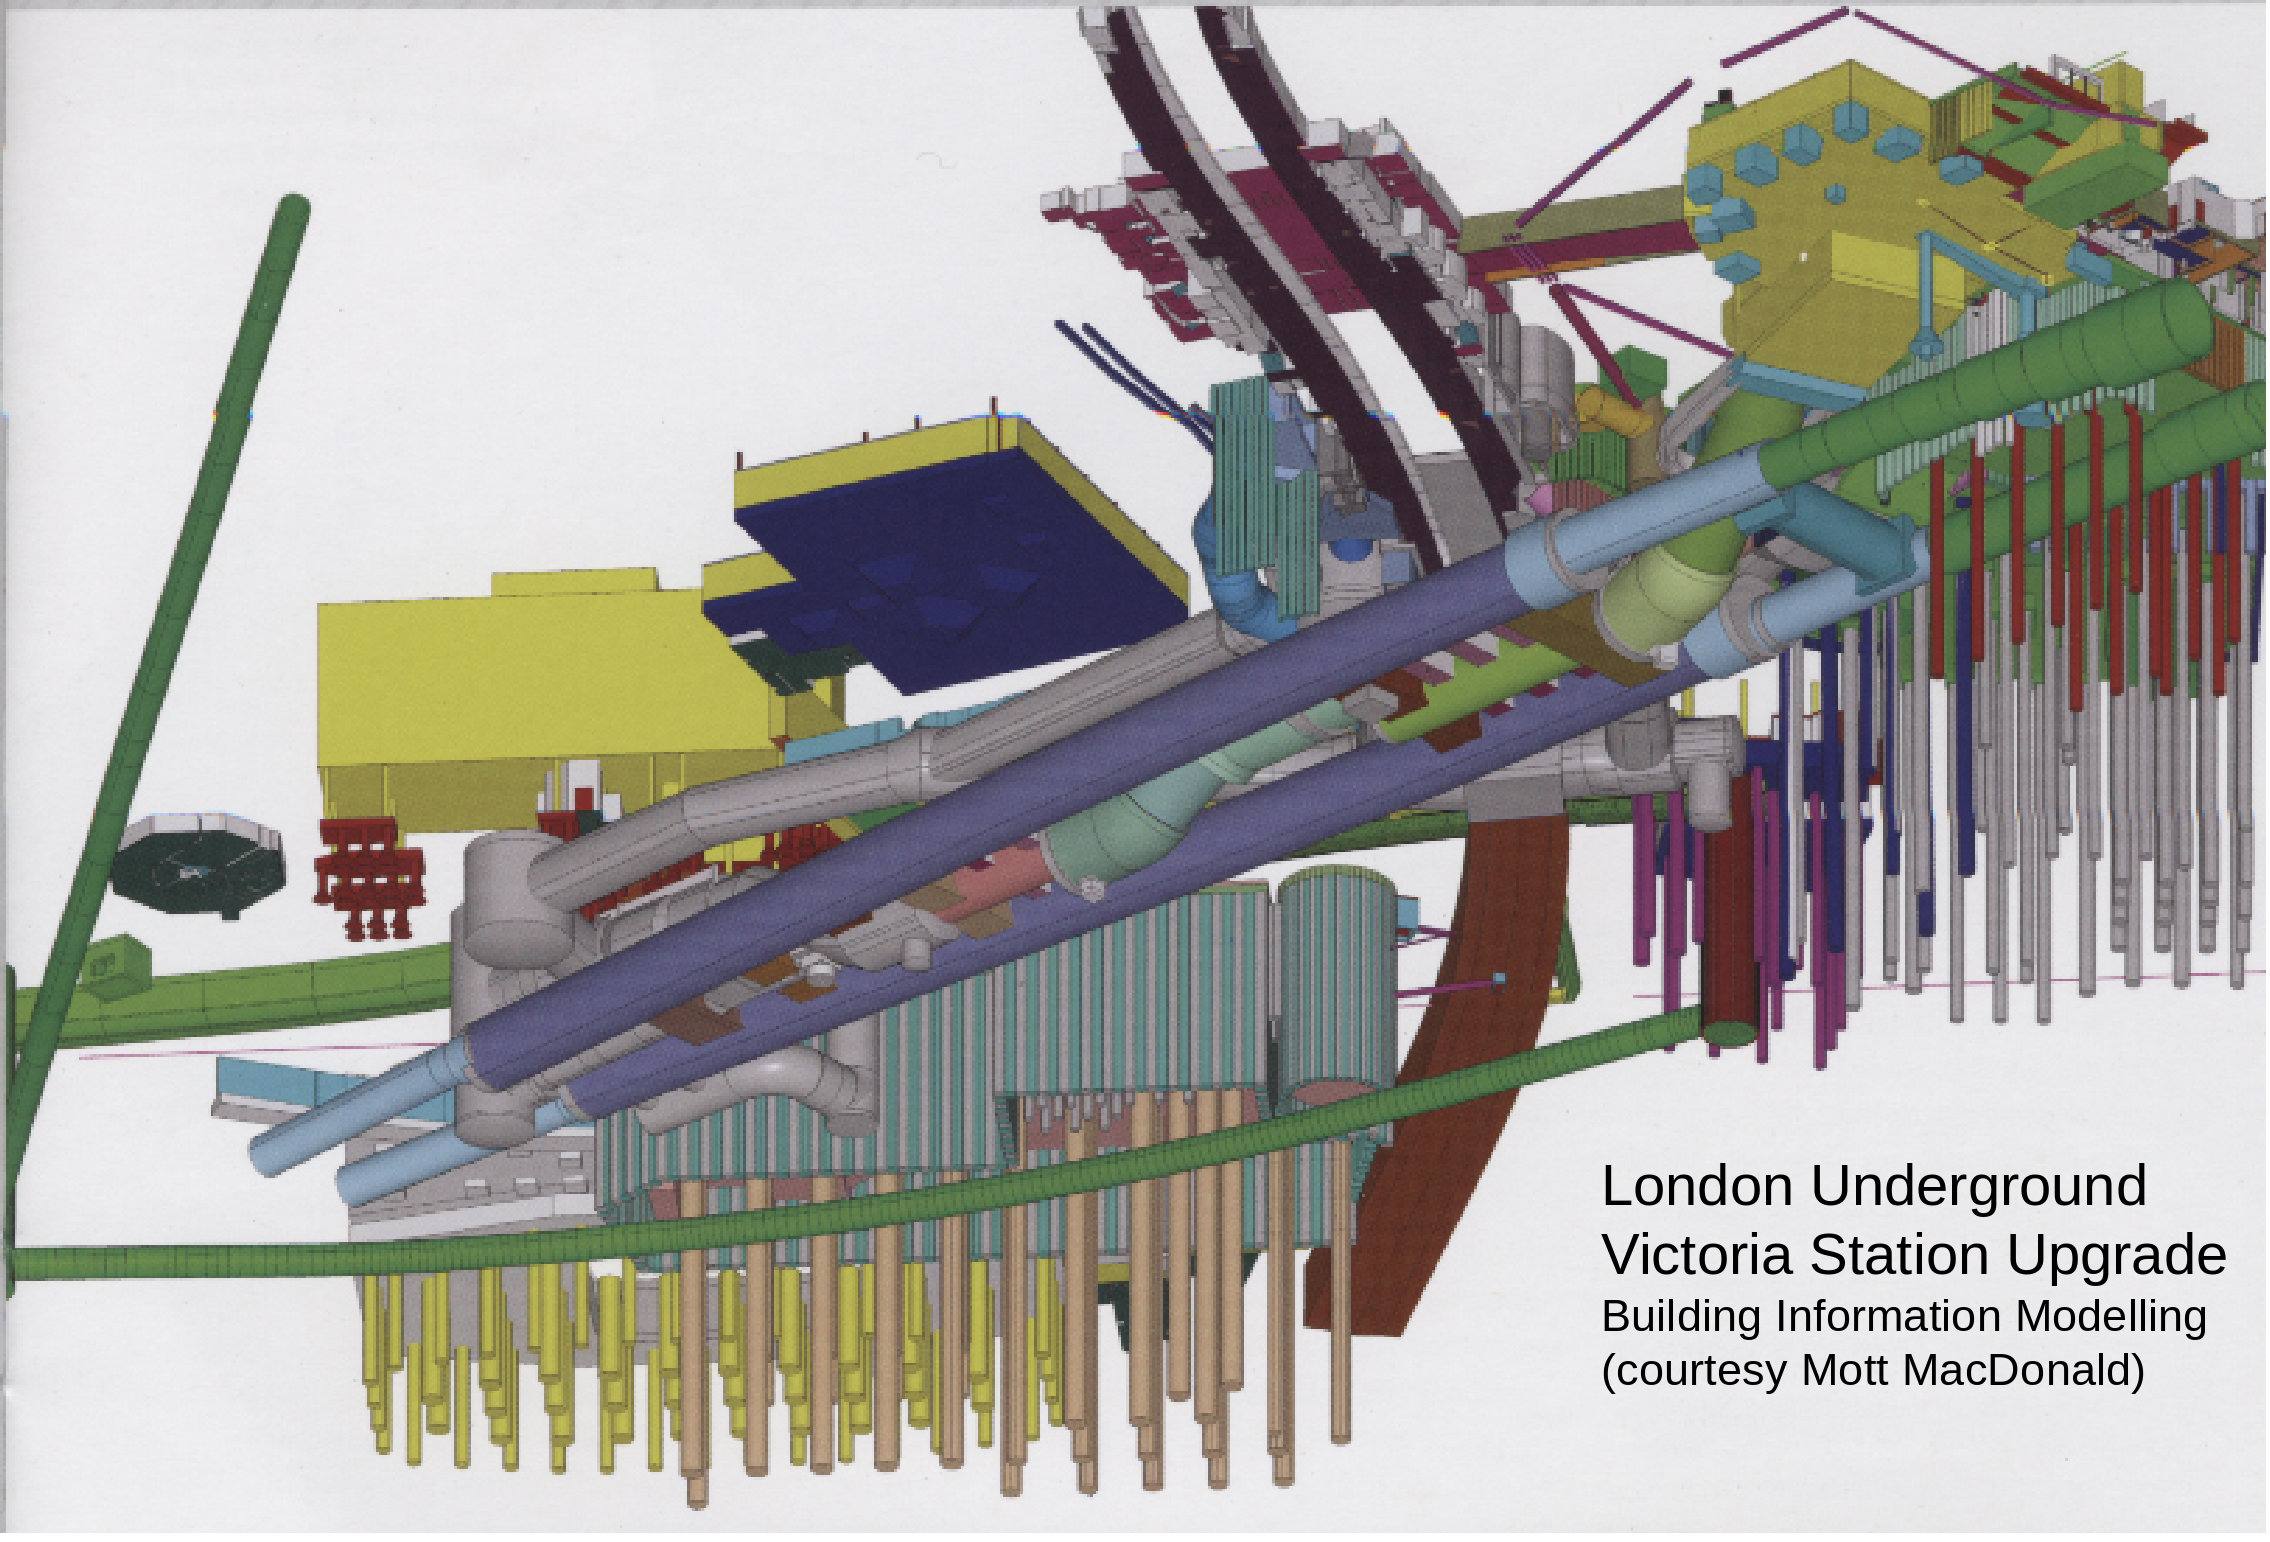
\includegraphics[width=0.85\textwidth]{figs/victoria-station.png}
	\caption{London Victoria station upgrade, London, UK}
\end{figure}
\end{frame}

%------------------------------------------------
\begin{frame}
\frametitle{Geotechnical modeling}
\begin{figure}
  \mode<beamer>{
	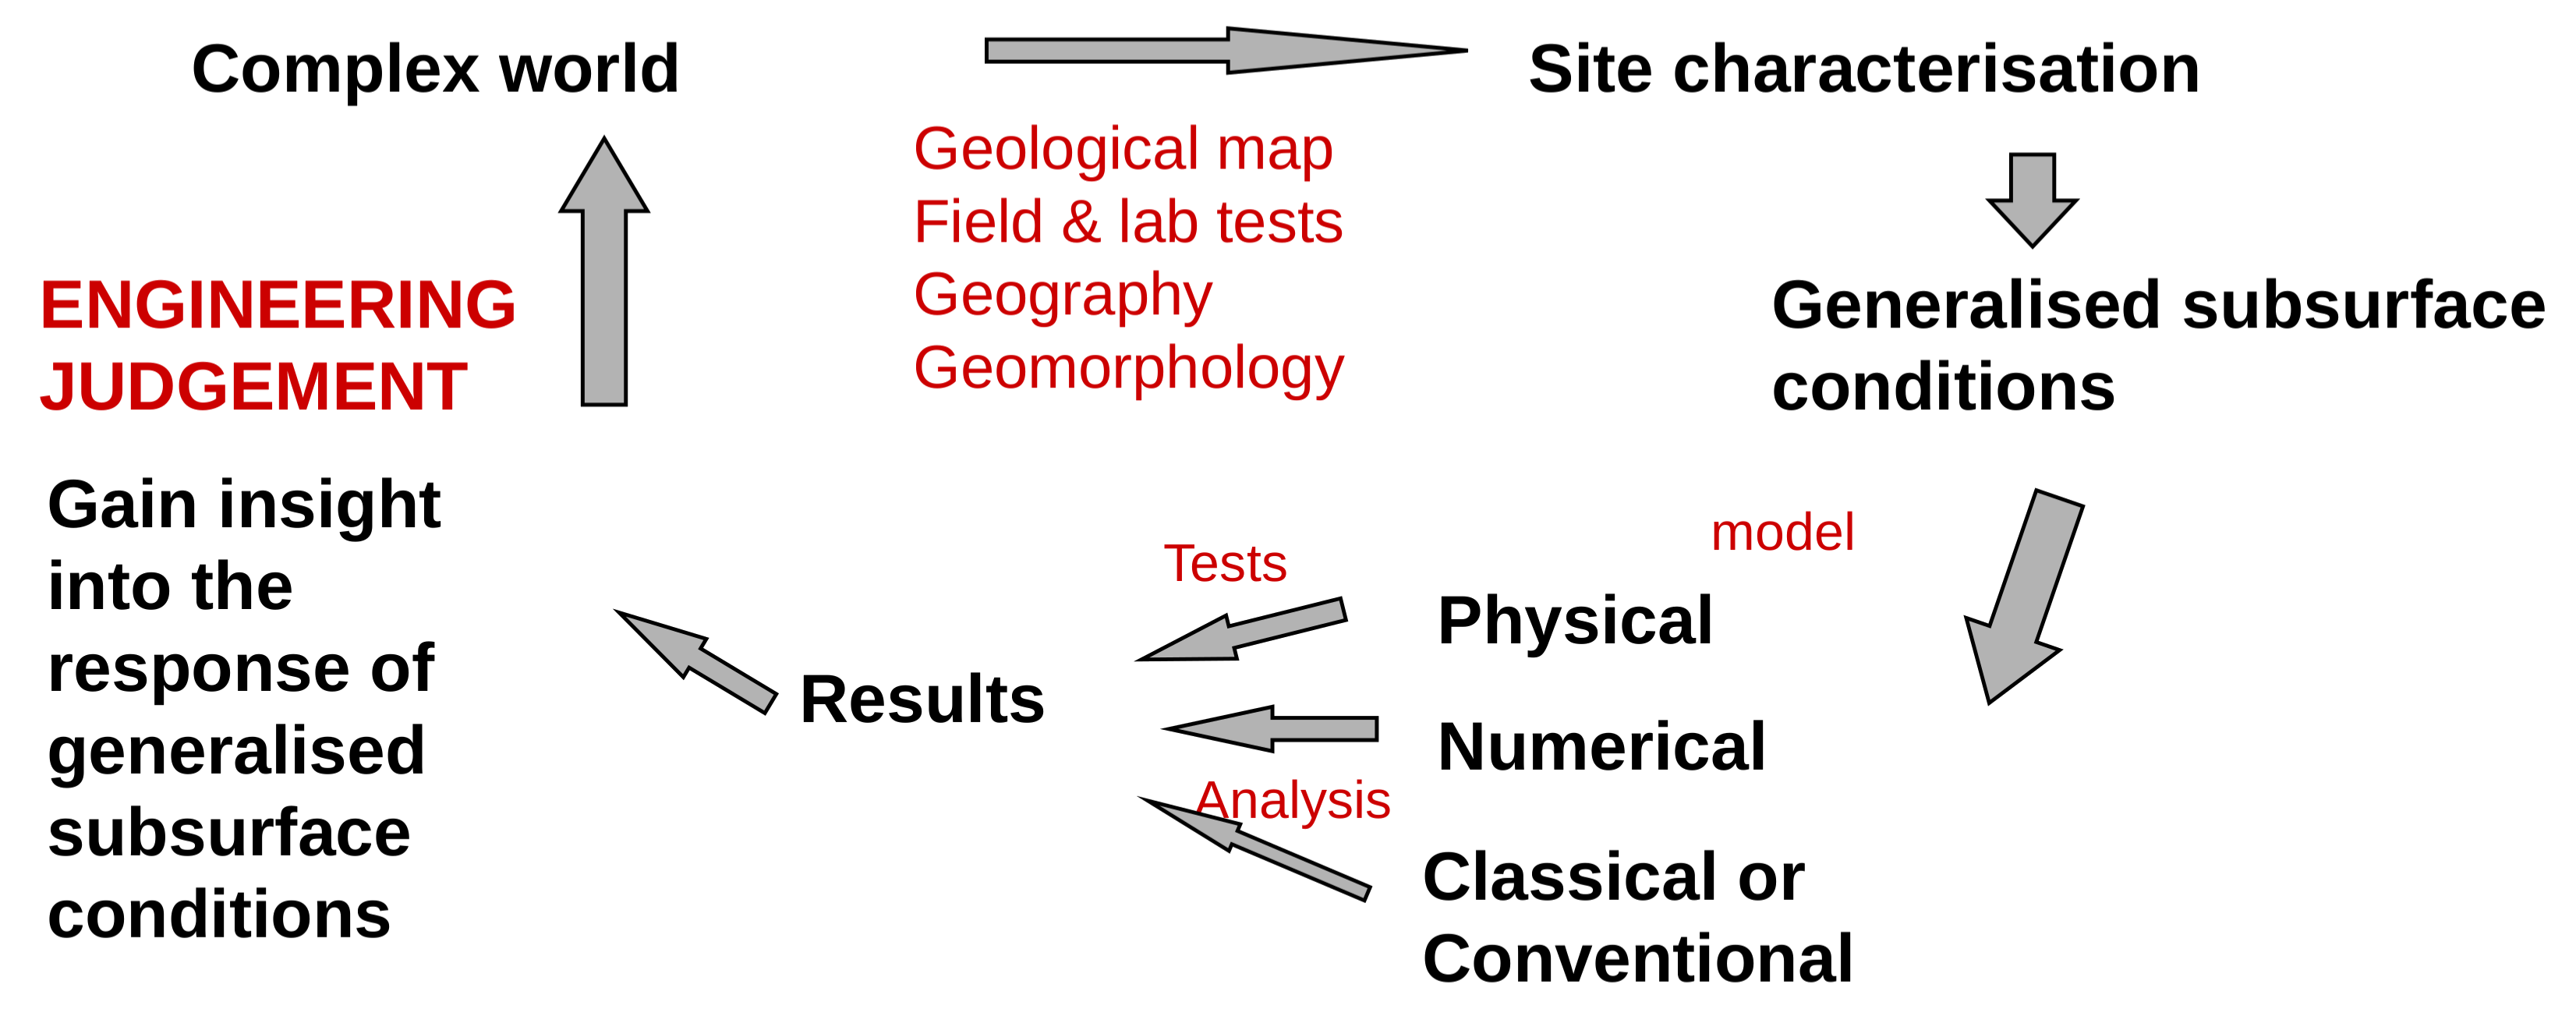
\includegraphics[width=0.95\textwidth]{figs/geotechnical-modeling-final.png}
  }
  \mode<handout>{
	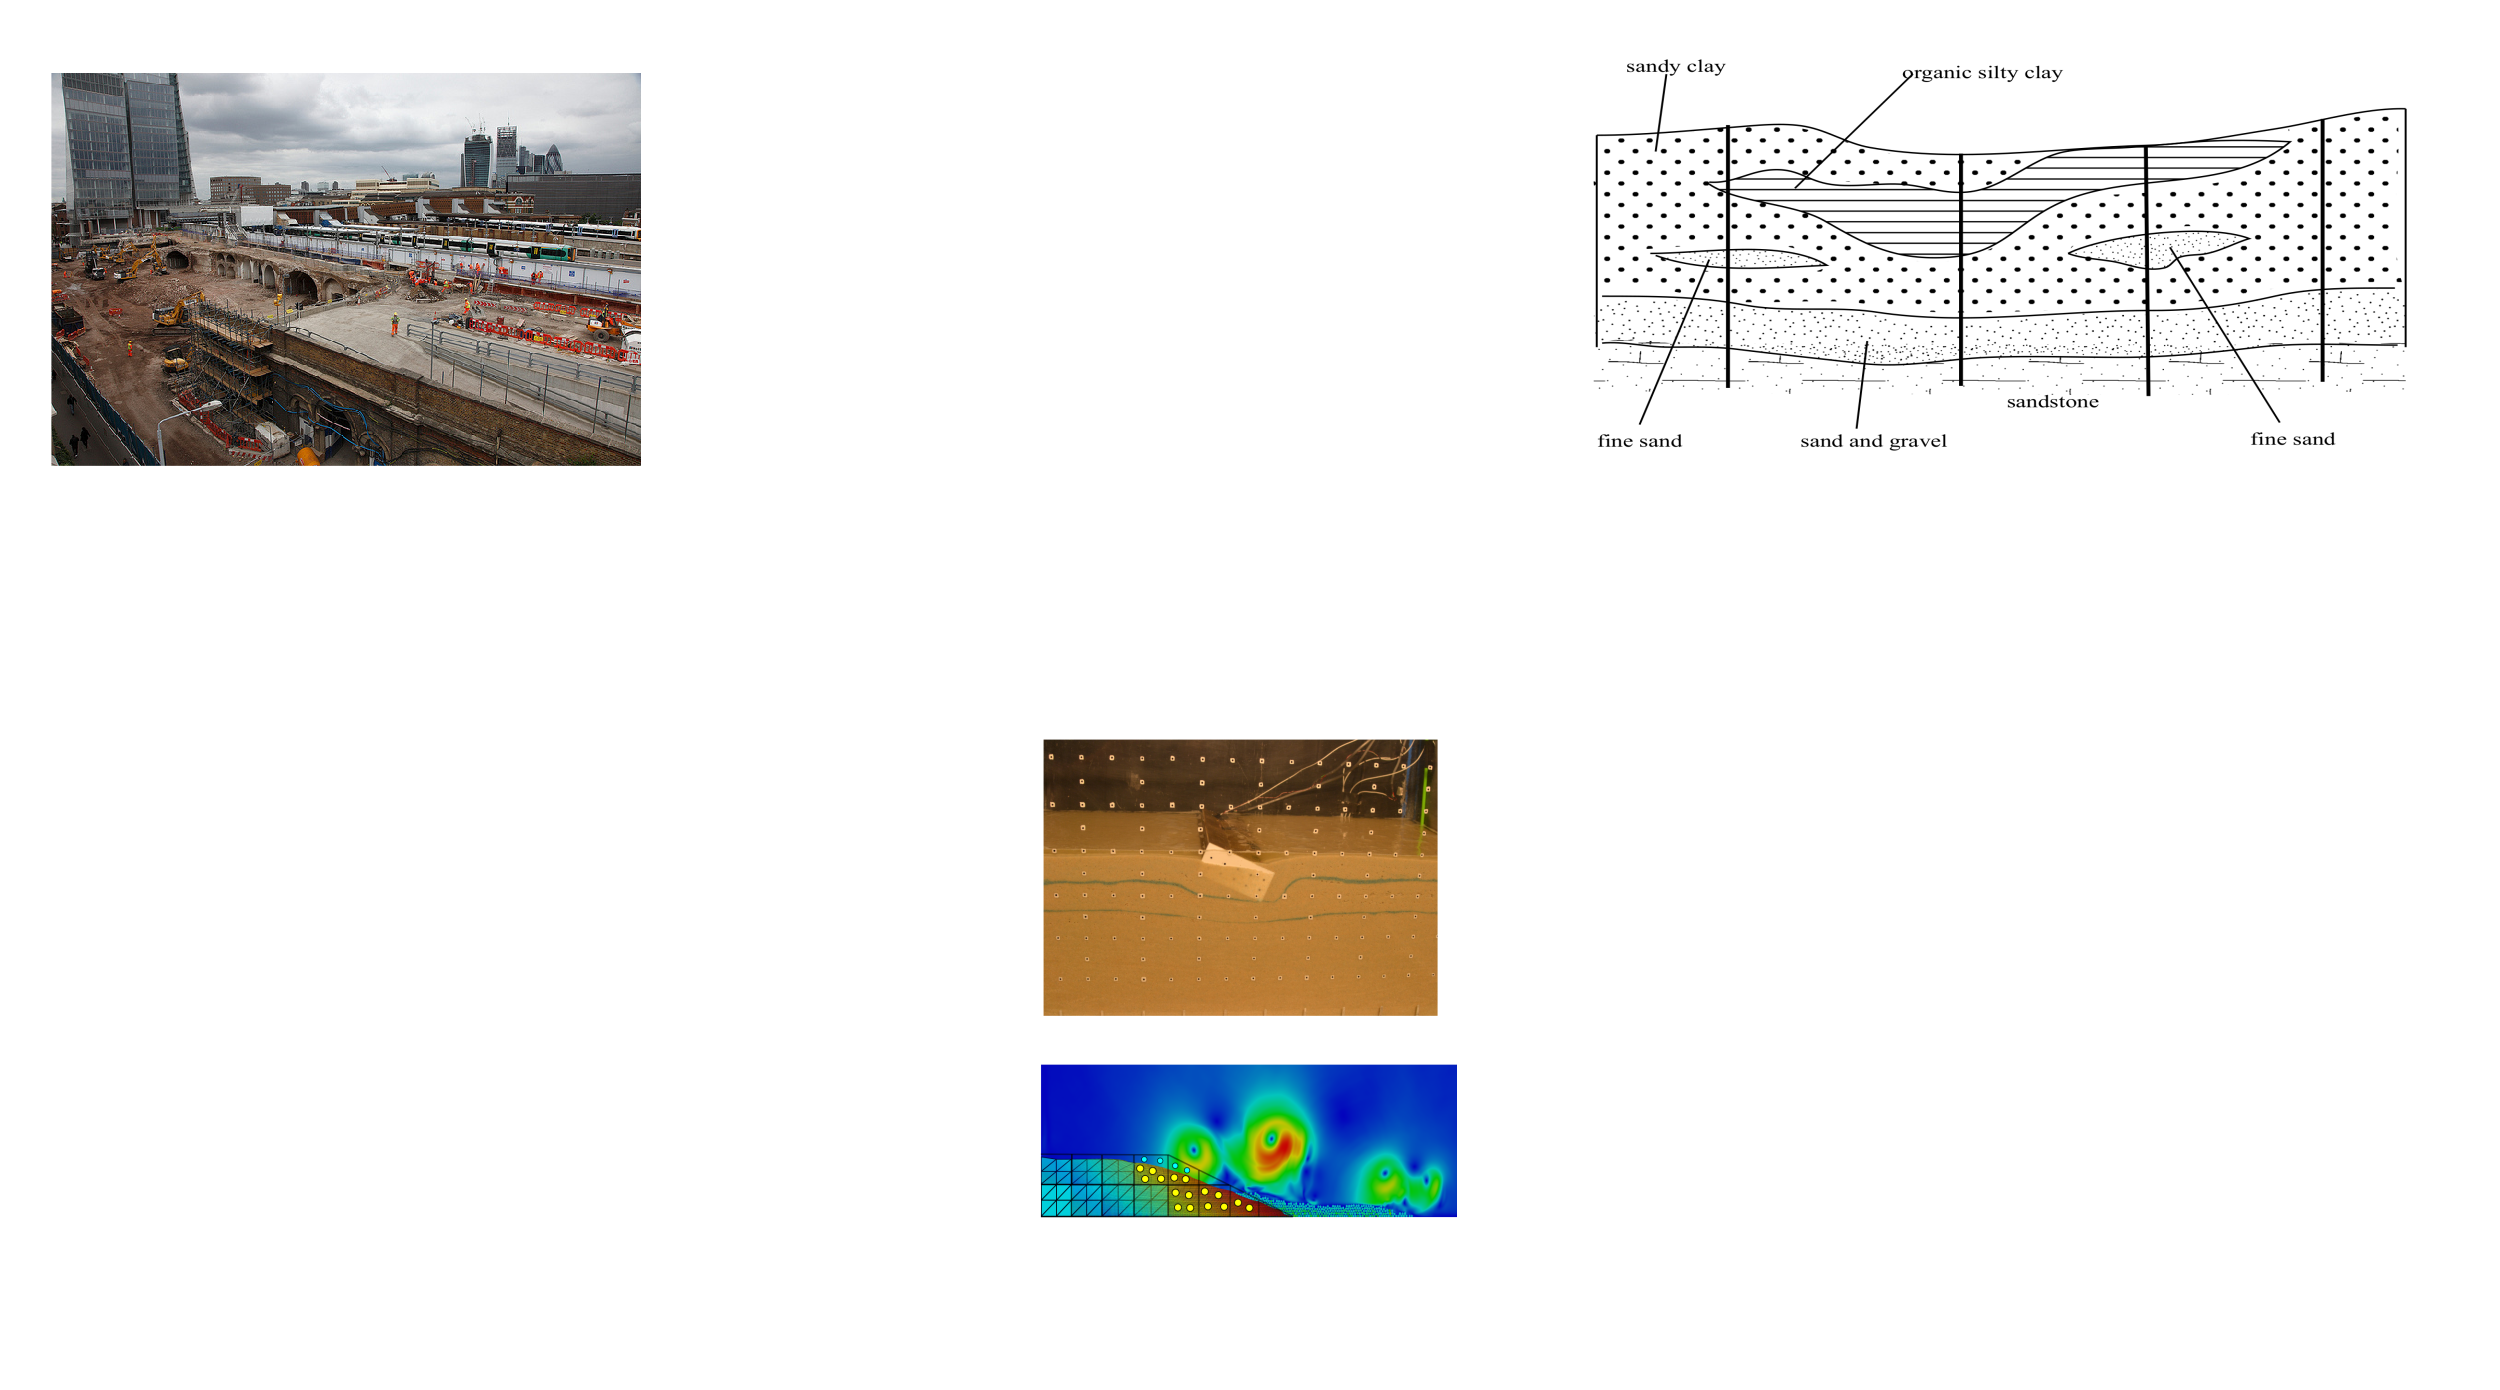
\includegraphics[width=0.95\textwidth]{figs/geotechnical-modeling.png}
  }
\end{figure}
\end{frame}

%------------------------------------------------
\begin{frame}
\frametitle{Soil behavior}
\begin{itemize}
	\item nonhomogeneous,
	\item anisotropic, 
	\item non-linear, 
	\item initial stress conditions, 
	\item stress history
	\item Geometry - very complex
\end{itemize}
\textbf{Soil Mechanics in practice - largely empirical}
\end{frame}

%------------------------------------------------
\begin{frame}
\frametitle{Geotechnical modeling: What should be modeled?}
\mode<beamer>{
\begin{itemize}
	\item Self weight effect of soils (This is why soil moves)
	\item Construction sequence (Complex geometry)
	\item Water movement (undrained, consolidation, drained)
	\item Insitu stresses (stiffness/strength depends on current stresses and stress history)
	\item Predict the ability of a design to withstand extreme loading conditions (you only have one chance)
\end{itemize}
}
\mode<handout>{
\vspace{4cm}
}
\begin{figure}
	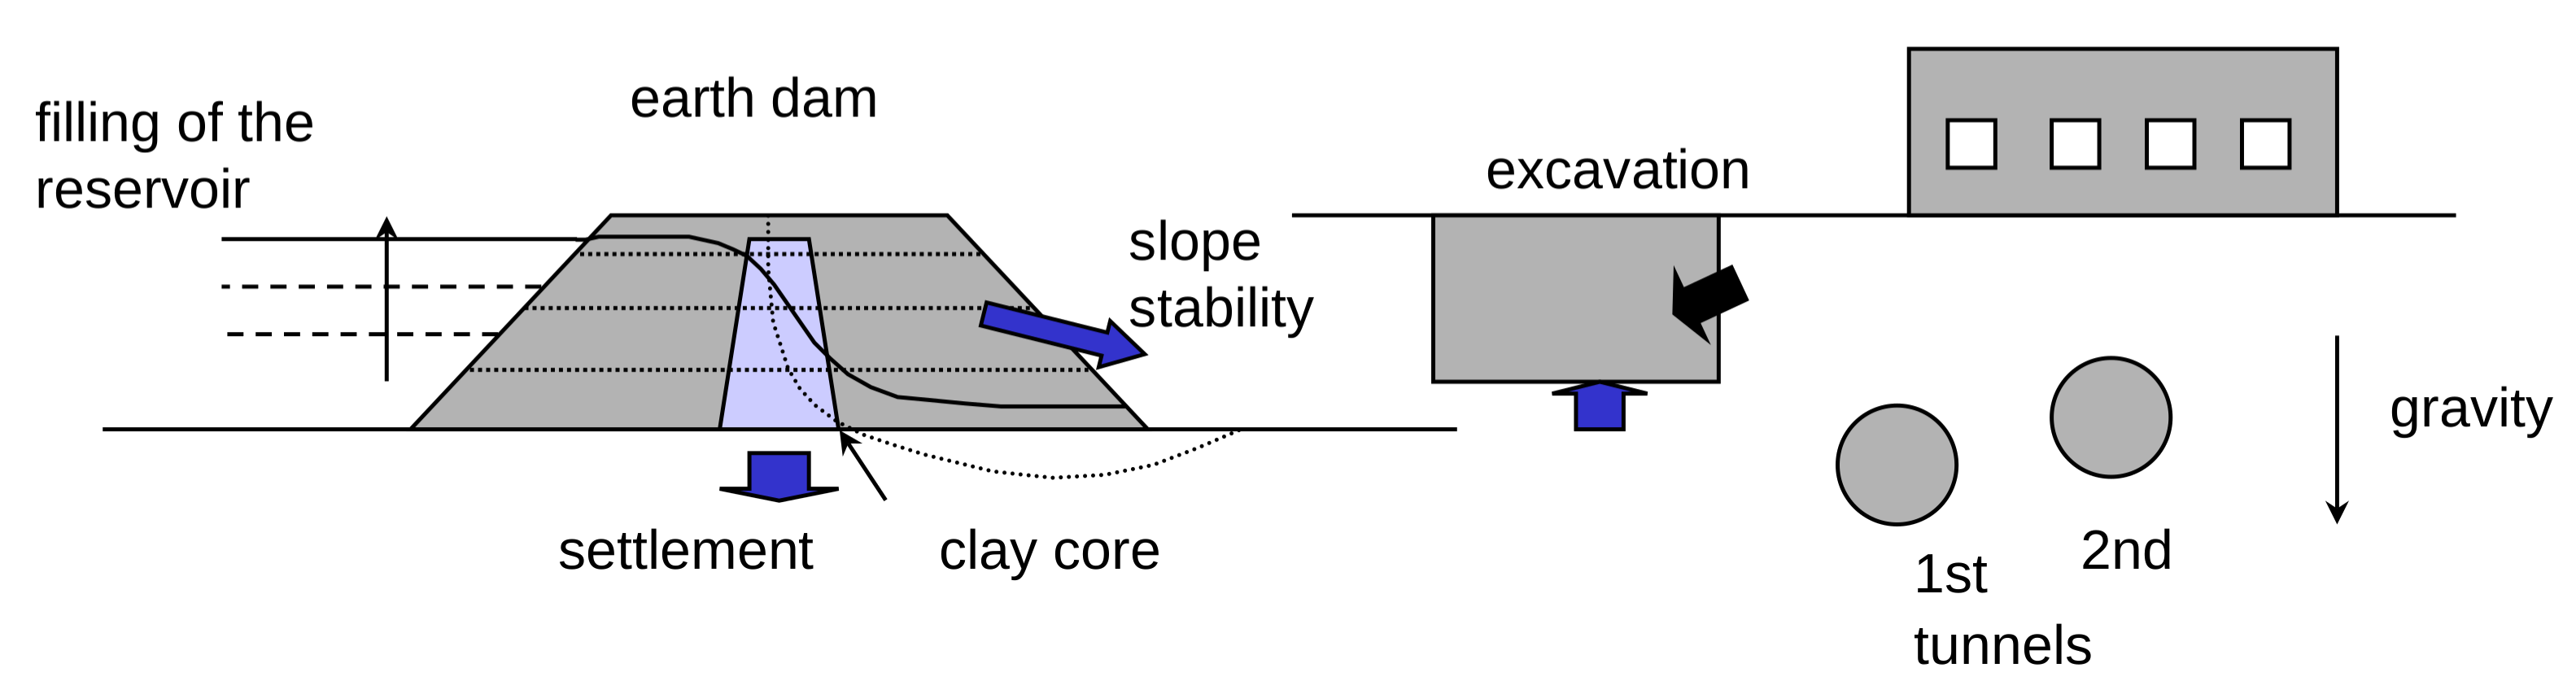
\includegraphics[width=0.95\textwidth]{figs/geotechnical-modeling-examples.png}
\end{figure}
\end{frame}

\section{Numerical methods for differential equations}
\subsection{Direct method}
%------------------------------------------------
\begin{frame}
\frametitle{Matrix analysis of structures}
\mode<beamer>{
	\begin{figure}
		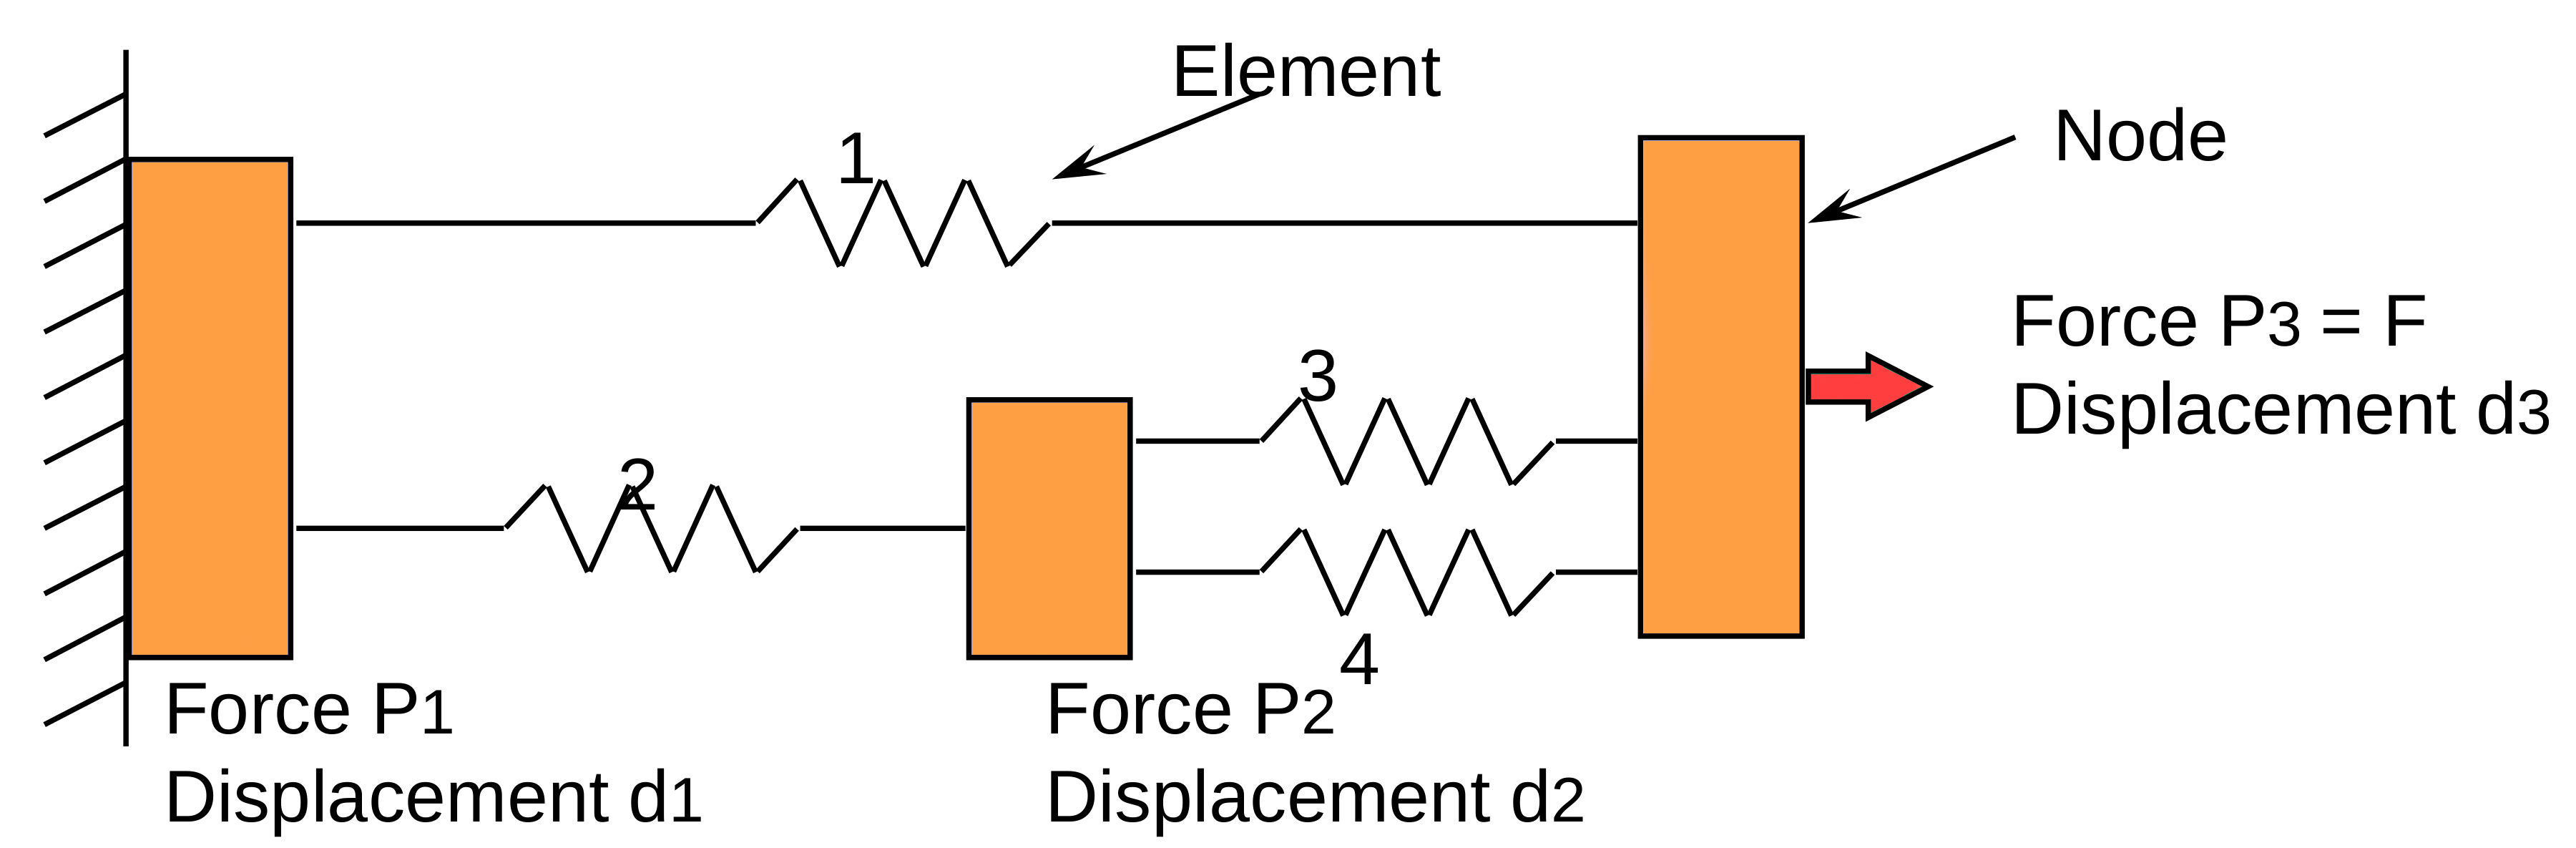
\includegraphics[width=0.95\textwidth]{figs/matrix-analysis-structures-final.png}
	\end{figure}
}
\mode<handout>{
	\begin{figure}
		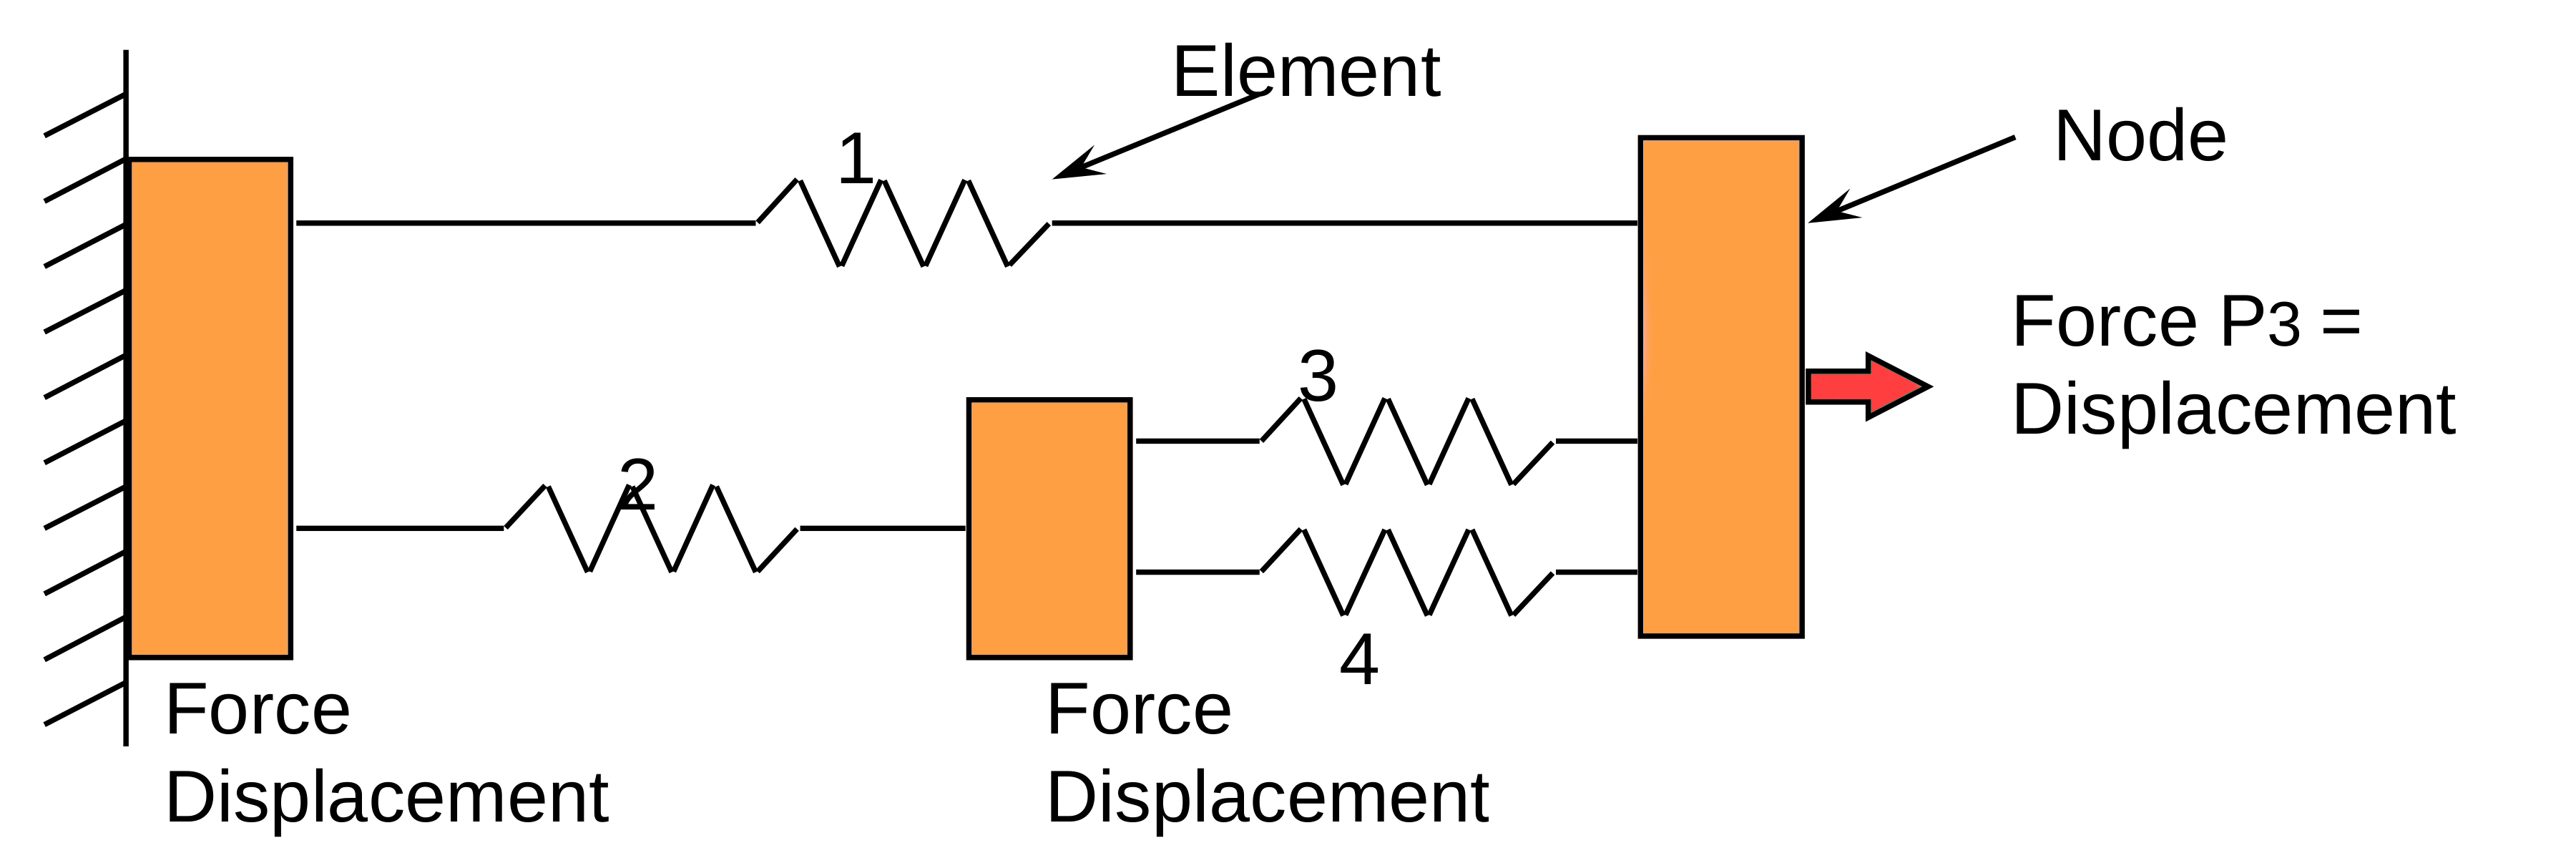
\includegraphics[width=0.95\textwidth]{figs/matrix-analysis-structures.png}
	\end{figure}
}

\begin{itemize}
	\item What are the known variables? \mode<beamer>{$d_1=0, P_2=0, P_3=F$(constant)}
	\item What are the unknowns? \mode<beamer>{$P_1, d_2, d_3$}
	\item What do we know? \mode<beamer>{Force or distortion relations at an element level.}
\end{itemize}
\end{frame}

%------------------------------------------------
\begin{frame}
\frametitle{Matrix analysis of structures: Equilibrium}
\mode<handout>{\vspace{1cm}}
\mode<beamer>{A structure is considered to be in equilibrium if, initially at rest, it remains 
	at rest when subjected to a system of forces and couples. If a structure is in equilibrium, 
	then all of its members and joints must also be in equilibrium.}
\begin{itemize}
	\item $P_1 = $\mode<beamer>{$-S_1 -S_2$}
	\item What are the unknowns? \mode<beamer>{$P_1, d_2, d_3$}
	\item What do we know? \mode<beamer>{Force or distortion relations at an element level.}
\end{itemize}

\mode<beamer>{
\begin{equation*}
\begin{bmatrix}
P_1 \\
P_2 \\
P_3 \\
\end{bmatrix} = 
\begin{bmatrix}
-1 & -1 &  0 &  0 \\
 0 &  1 & -1 & -1 \\
 1 &  0 &  1 &  1 \\
\end{bmatrix} + 
\begin{bmatrix}
S_1 \\
S_2 \\
S_3 \\
s_4 \\
\end{bmatrix}
\end{equation*}

\begin{equation*}
\mathbf{P} = \mathbf{A^T} \mathbf{S}
\end{equation*}
}

\mode<handout>{
	\vspace{2cm}
}
\end{frame}


%------------------------------------------------
\begin{frame}
\frametitle{Matrix analysis of structures: Compatibility}
\mode<handout>{\vspace{4cm}}
\mode<beamer>{
\begin{itemize}
	\item compatibility relates the deformations of a structure so that its
	various parts (members, joints, and supports) fit together without any gaps or
	overlaps. 
	\item ensure that the deformed shape of the structure is continuous (except at the 
	locations of any internal hinges or rollers), and is consistent with the support
	conditions.
\end{itemize}
}
\end{frame}

%------------------------------------------------
\begin{frame}
\frametitle{Matrix analysis of structures: Compatibility}
$v$ = internal spring distortion
$\delta$ = nodal displacement
\begin{itemize}
	\item $v_1 = $\mode<beamer>{$d_3 - d_1$}
	\item $v_2 = $\mode<beamer>{$d_2 - d_1$}
	\item $v_3 = $\mode<beamer>{$d_3 - d_2$}
	\item $v_4 = $\mode<beamer>{$d_3 - d_2$}
\end{itemize}


\mode<beamer>{
	\begin{equation*}
	\begin{bmatrix}
	v_1 \\
	v_2 \\
	v_3 \\
	v_4 \\
	\end{bmatrix} = 
	\begin{bmatrix}
	-1 &  0 &  1 \\
 	-1 &  1 &  0 \\
	 0 & -1 &  1 \\
	 0 & -1 &  1 \\
	\end{bmatrix} + 
	\begin{bmatrix}
	d_1 \\
	d_2 \\
	d_3 \\
	\end{bmatrix}
	\end{equation*}
	
	\begin{equation*}
	\mathbf{v} = \mathbf{A} \mathbf{d}
	\end{equation*}
}

\mode<handout>{
	\vspace{3cm}
}
\end{frame}

%------------------------------------------------
\begin{frame}
\frametitle{Matrix analysis of structures: Physical condition}
Force-distance relationship: spring constant

\begin{center}
	\begin{tabular}{l l l l l}
		\toprule
		\textbf{spring \#} & 1 & 2 & 3 & 4 \\
		\textbf{stiffness ($F.L^{-1}$)} & 3 & 2 & 1 & 2 \\
		\bottomrule
	\end{tabular}
\end{center}

\mode<beamer>{
	\begin{equation*}
	\begin{bmatrix}
	S_1 \\
	S_2 \\
	S_3 \\
	S_4 \\
	\end{bmatrix} = 
	\begin{bmatrix}
	3 & 0 & 0 & 0 \\
	0 & 2 & 0 & 0 \\
	0 & 0 & 1 & 0 \\
	0 & 0 & 0 & 2 \\
	\end{bmatrix}
	\begin{bmatrix}
	v_1 \\
	v_2 \\
	v_3 \\
	v_4 \\
	\end{bmatrix}
	\end{equation*}
	
	\begin{equation*}
	\mathbf{s} = \mathbf{D} \mathbf{v}
	\end{equation*}
}

\mode<handout>{
	\vspace{3cm}
}
\end{frame}

%------------------------------------------------
\begin{frame}
\frametitle{Matrix analysis of structures: Direct Method}
Combine all the equations:
$\mathbf{P}$ = \mode<beamer>{$\mathbf{A^TS = A^TDv = A^TDAd = Kd}$}

where $\mathbf{K}$ = \mode<beamer>{$A^T D A $ (Global stiffness matrix)}
\mode<beamer>{
\begin{align*} 	
K & = 
\begin{bmatrix}
-1 & -1 &  0 &  0 \\
0 &  1 & -1 & -1 \\
1 &  0 &  1 &  1 \\
\end{bmatrix}
\begin{bmatrix}
3 & 0 & 0 & 0 \\
0 & 2 & 0 & 0 \\
0 & 0 & 1 & 0 \\
0 & 0 & 0 & 2 \\
\end{bmatrix}
\begin{bmatrix}
-1 &  0 &  1 \\
-1 &  1 &  0 \\
0 & -1 &  1 \\
0 & -1 &  1 \\
\end{bmatrix} \notag \\%
%
%
 &= 
 \begin{bmatrix}
  5 & -2 & -3 \\
 -2 &  5 & -3 \\
 -3 & -3 &  6 \\
 \end{bmatrix} \\%
%
%
\begin{bmatrix}
P_1 \\
P_2 \\
P_3 \\
\end{bmatrix}
& =
\begin{bmatrix}
5 & -2 & -3 \\
-2 &  5 & -3 \\
-3 & -3 &  6 \\
\end{bmatrix}
\begin{bmatrix}
d_1 \\
d_2 \\
d_3 \\
\end{bmatrix}
\end{align*}
Apply Boundary conditions $d_1=0$, $P_2=0$ and $P_3=F$ and solve $P_1$, $d_2$ and $d_3$
}

\mode<handout>{
	\vspace{6cm}
}
\end{frame}

%------------------------------------------------
\begin{frame}
\frametitle{Matrix analysis of structures}
\begin{figure}
	\mode<beamer>{
		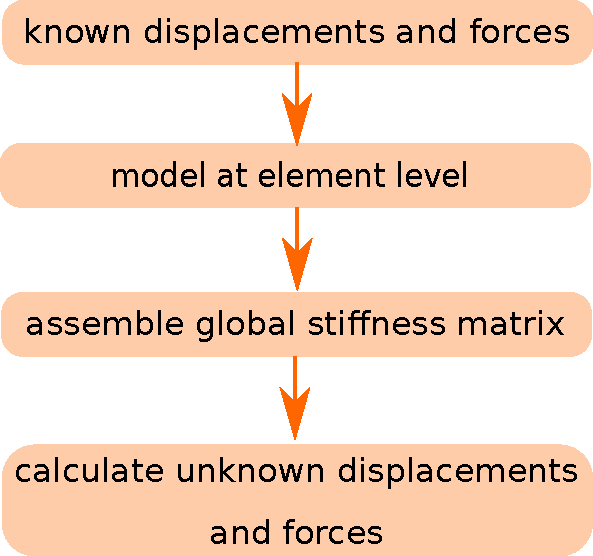
\includegraphics[width=0.6\textwidth]{figs/computational-workflow.pdf}
	}
	\mode<handout>{
		\vspace{5cm}
	}
\end{figure}
\end{frame}

%------------------------------------------------
\begin{frame}
\frametitle{Numerical analysis of engineering problems}
\mode<beamer>{
\begin{itemize}
	\item Conceptualize the system
	\begin{itemize}
		\item Geometry
		\item Properties
		\item Processes
	\end{itemize}
	\item Describe it mathematically
	\begin{itemize}
		\item Select the relevant differential equations
	\end{itemize}
	\item Solve the equations (numerically)
	\begin{itemize}
		\item Discretize the system
		\item Settle for approximations (numerical techniques)
	\end{itemize}
	\item Interpret the results
\end{itemize}	
}
\mode<handout>{
	\vspace{5cm}
}
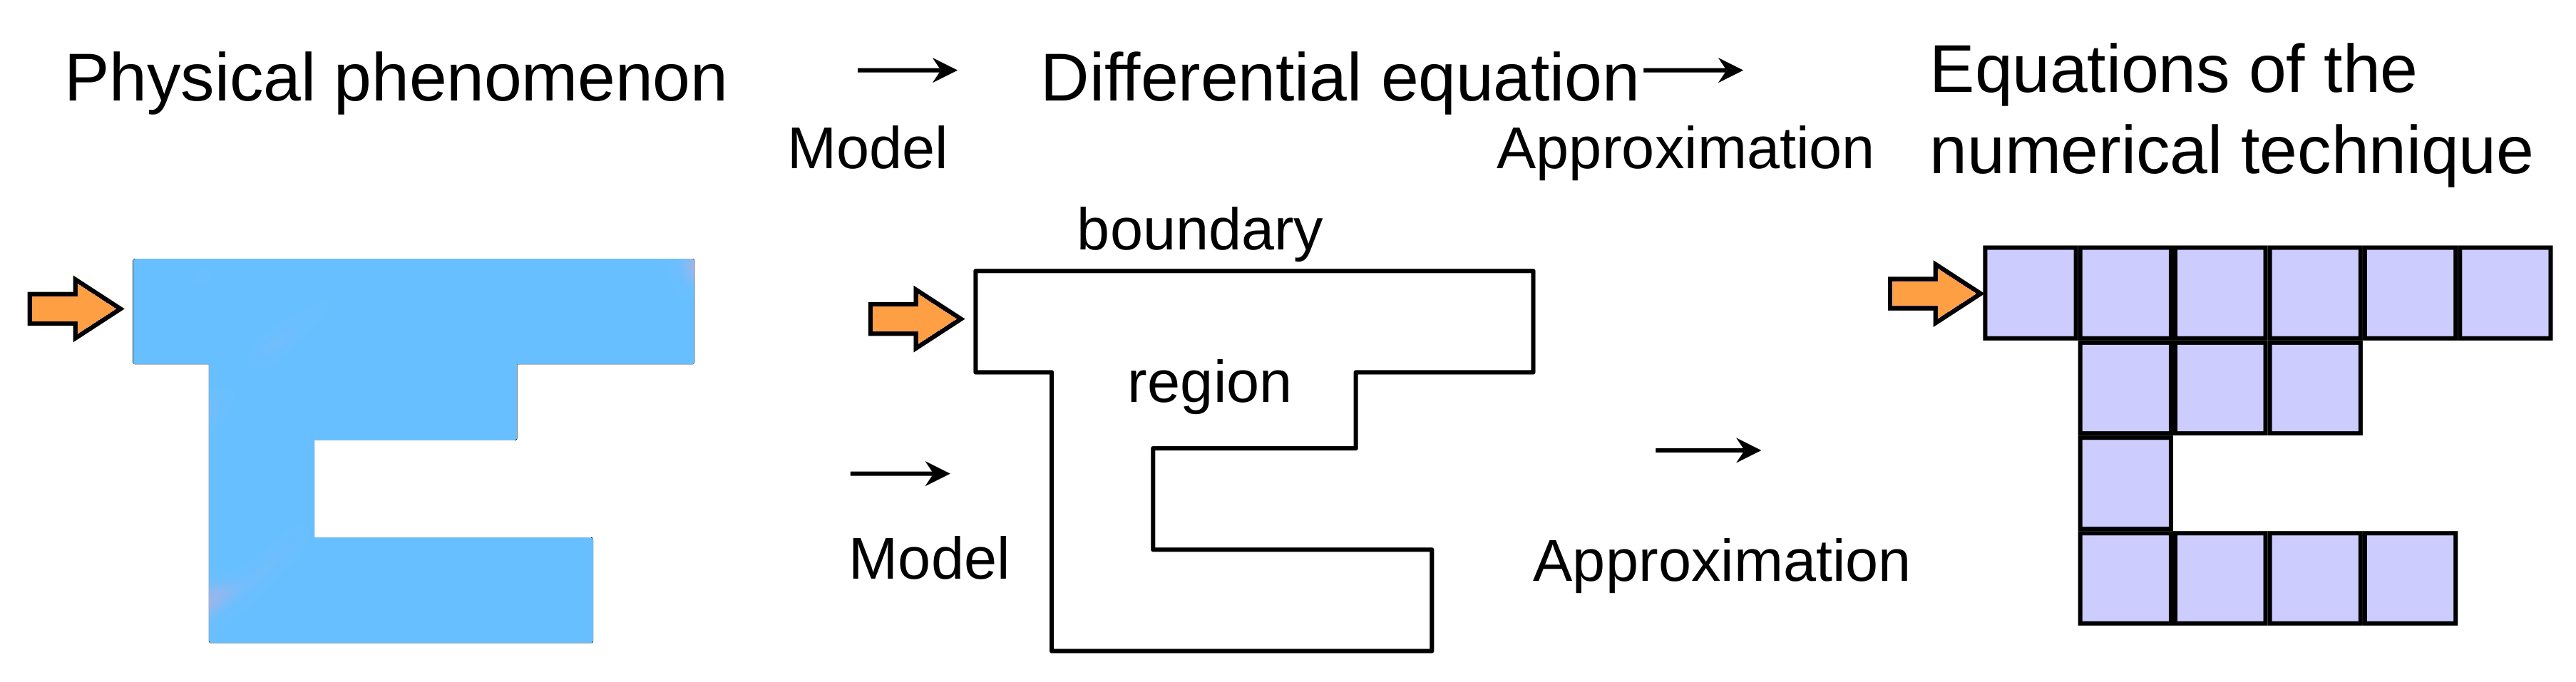
\includegraphics[width=\textwidth]{figs/numerical-pde-workflow.png}
\end{frame}

%------------------------------------------------
\begin{frame}
\frametitle{Boundary value problems}

Differential equations coupled with boundary conditions

\begin{itemize}
	\item Steady state (time-independent)
\mode<beamer>{
	\begin{itemize}
		\item Static load-deformation problems: 
		$\partial \sigma / \partial x = 0$ (force + disp. B.C)
		\item Steady seepage state, flow problems: 
		$\partial q / \partial x = 0$ (head + flow B.C)
	\end{itemize}
}
\mode<handout>{
\vspace{2cm}
}
	\item Transient (time-dependent)
\mode<beamer>{
	\begin{itemize}
		\item Consolidation/pore-fluid migration/multiphase flows
		\item Dynamic loading (earthquakes, wave actions)
		\item Contaminant transport processes
	\end{itemize}
}
\mode<handout>{
\vspace{2cm}
}
	\end{itemize}	
\end{frame}

\end{document} 
